\documentclass{../industrial-development}
\graphicspath{{07-version-control-system/}}

\title{Использование систем управления версиями в промышленной разработке}
\author{Заплатин Егор Сергеевич, ПИ-21 МО}
\date{}

\begin{document}

\begin{frame}
  \titlepage
\end{frame}

\begin{frame}{План лекции}
  \tableofcontents
\end{frame}

\section{Введение}

\subsection{Что такое система управления версиями}

\begin{frame} \frametitle{Что такое система управления версиями}
  \begin{block}{Определение}
    \alert{Системы контроля версий} --- это категория программных инструментов, которые помогают команде программного обеспечения управлять изменениями исходного кода с течением времени
  \end{block}
  
  \begin{itemize}
  \item Каждая модификация кода отслеживается в специальном виде в базе данных
  \item При обнаружении ошибки можно «повернуть время вспять», сравнить исходный код с предыдущими версиями
  \end{itemize}
\end{frame}

\lecturenotes

Контроль версий помогает отслеживать каждое индивидуальное изменение каждым вкладчиком, помогает предотвратить конфликты при параллельной работе. Изменения, внесенные в одну часть программного обеспечения, могут быть несовместимы с изменениями, внесенными другим разработчиком, работающим параллельно. Эта проблема должна быть обнаружена и решена упорядоченным образом, не блокируя работу остальной команды. Кроме того, во всех разработках программного обеспечения любое изменение может вводить новые ошибки, и новому коду нельзя доверять, пока он не будет протестирован. Поэтому тестирование и разработка продолжаются до тех пор, пока не будет готова новая версия~\cite{Atlassian}.

\subsection{Преимущества систем контроля версий}

\begin{frame} \frametitle{Преимущества систем контроля версий}

  \begin{itemize}
  \item Полная долгосрочная история изменений каждого файла
  \item Ветвление и слияние
  \item Отслеживаемость
  \end{itemize}
\end{frame}

\begin{frame} \frametitle{Полная долгосрочная история изменений каждого файла}

  \begin{itemize}
  \item Сохранются все изменения каждого файла, сделанные многими людьми на протяжении долгих лет
  \item Каждое изменение включает в себя автора, дату и письменные заметки о целях изменения
  \end{itemize}
\end{frame}

\lecturenotes

Имеются ввиду все изменения, сделанные многими людьми на протяжении многих лет. Изменения включают в себя создание и удаление файлов, а также редактирование их содержимого. Различные инструменты VCS отличаются тем, насколько хорошо они могут обрабатывать переименование и перемещение файлов. Эта история должна также включать автора, дату и письменные заметки о целях каждого изменения. Наличие полной истории позволяет вернуться к предыдущим версиям, помогает в анализе причин ошибок, и это важно, когда нужно исправлять проблемы в более старых версиях программного обеспечения. Если программное обеспечение активно разрабатывается, почти все можно считать «более старой версией» программного обеспечения~\cite{Atlassian}.

\begin{frame} \frametitle{Ветвление и слияние}
  
  \begin{itemize}
  \item Возможность создания веток позволяет нескольким разработчикам работать над одним проектом независимо друг от друга
  \item Ветки можно объединять воедино, сливая сделанные изменения
  \item Предоставляется интерфейс для разрешения конфликтов при слиянии
  \end{itemize}
\end{frame}

\lecturenotes

Наличие членов команды работающих параллельно не простая ситуация, но даже люди, работающие самостоятельно, могут извлечь выгоду из способности работать над независимыми потоками изменений. Создание «ветки» в инструментах VCS позволяет нескольким потокам работать независимо друг от друга, а также предоставляет возможность объединить эту работу вместе, позволяя разработчикам проверять, что изменения в каждой ветке не конфликтуют. Многие команды программного обеспечения применяют практику ветвления для каждой функции или ветвления для каждой версии, или и то, и другое. Существует множество различных рабочих процессов, которые команды могут выбирать, когда они решают, как использовать ветвление и объединяющие объектов в VCS~\cite{Atlassian}.

\begin{frame} \frametitle{Отслеживаемость}
 
  \begin{itemize}
  \item Всегда можно понять когда и зачем код был написан
  \item Легко проводить анализ причинно-следственных связей
  \end{itemize}
\end{frame}

\lecturenotes

Возможность отслеживать каждое изменение, внесенное в программное обеспечение, и подключать его к программам управления проектами и программам отслеживания ошибок, таким как Jira, возможность комментировать каждое изменение сообщением, описывающим цель и намерение изменения, может помочь не только при анализе причинно-следственных связей и других экспертиз. Имея под рукой аннотированную историю кода, можно прочитать код, пытаясь понять, что он делает и почему он так сконструирован. Это может позволяет разработчикам делать правильные и гармоничные изменения, соответствующие намеченному долгосрочному дизайну системы. Это может быть особенно важно для эффективной работы с устаревшим кодом и имеет решающее значение для того, чтобы разработчики могли оценивать будущую работу с любой точностью~\cite{Atlassian}.

\section{Виды систем контроля версий}

\subsection{Централизованные системы контроля версий}

\begin{frame} \frametitle{Централизованные системы контроля версий}
  \begin{block}{Определение}
    В \alert{централизованных системах контроля версий} есть центральный сервер, на котором хранятся все файлы под версионным контролем, и ряд клиентов, которые получают копии файлов 
из него
  \end{block}
 
\end{frame}

\begin{frame} \frametitle{Схема централизованного контроля версий}
  \centerline{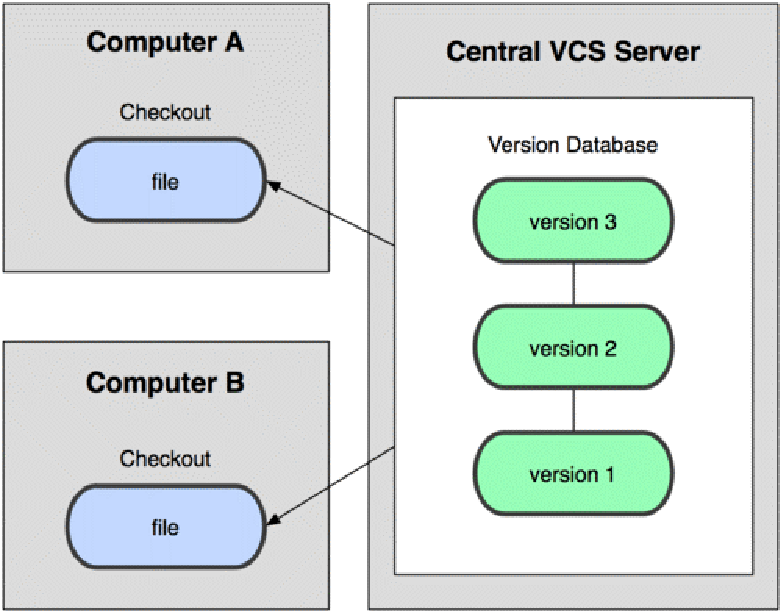
\includegraphics[width=0.7\textwidth]{centralizedVCS.pdf}}
\end{frame}

\begin{frame} \frametitle{Особенности централизованных систем контроля версий}
  \begin{itemize}
  \item Удобное администрирование: администраторы имеют четкий контроль над тем, кто и что может делать
  \item Центральный сервер является уязвимым местом всей системы, при его повреждении можно потерять всю историю проекта
  \end{itemize}
\end{frame}

\lecturenotes

Такой подход имеет множество преимуществ. К примеру, все знают, кто и чем занимается в проекте. У администраторов есть чёткий контроль над тем, кто и что может делать, и, конечно, администрировать ЦСКВ намного легче, чем локальные базы на каждом клиенте.

Однако при таком подходе есть и несколько серьёзных недостатков. Наиболее очевидный — централизованный сервер является уязвимым местом всей системы. Если сервер выключается на час, то в течение часа разработчики не могут взаимодействовать, и никто не может сохранить новой версии своей работы. Если же повреждается диск с центральной базой данных и нет резервной копии, вы теряете абсолютно всё — всю историю проекта, разве что за исключением нескольких рабочих версий, сохранившихся на рабочих машинах пользователей~\cite[с.~6--7]{ProGit}.

\subsection{Распределённые системы контроля версий}

\begin{frame} \frametitle{Распределённые системы контроля версий}
  \begin{block}{Определение}
    В \alert{распределённых системах контроля версий} клиенты не просто выгружают последние версии файлов, а полностью копируют весь репозиторий. Каждый раз, когда клиент забирает свежую версию файлов, он создаёт себе полную копию всех данных
  \end{block}
 
\end{frame}

\begin{frame} \frametitle{Схема распределённой системы контроля версий}
  \centerline{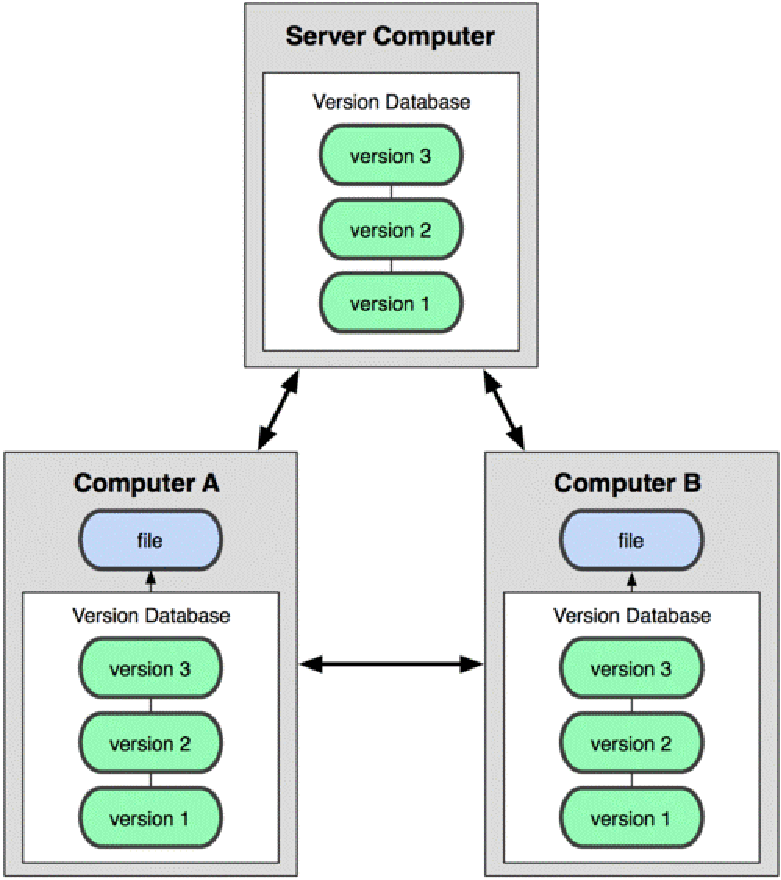
\includegraphics[width=0.5\textwidth]{distributedVCS.pdf}}
\end{frame}

\begin{frame} \frametitle{Особенности распределённых систем контроля версий}
  \begin{itemize}
  \item При повреждении удалённого сервера любой клиент может полностью восстановить базу данных
  \item Можно работать с несколькими удалёнными репозиториями, одновременно вести несколько типов рабочих процессов
  \end{itemize}
\end{frame}

\lecturenotes

В случае, когда «умирает» сервер, через который шла работа, любой клиентский репозиторий может быть скопирован обратно на сервер, чтобы восстановить базу данных. 

Кроме того, в большей части этих систем можно работать с несколькими удалёнными репозиториями, таким образом, можно одновременно работать по-разному с разными группами людей в рамках одного проекта. Так, в одном проекте можно одновременно вести несколько типов рабочих процессов, что невозможно в централизованных системах~\cite[с.~7]{ProGit}.

\section{Популярные системы контроля версий}

\subsection{Subversion}

\begin{frame} \frametitle{Subversion}
  \begin{block}{}
    \alert{Subversion (также известная как «SVN»)} --- свободная централизованная система управления версиями, официально выпущенная в 2004 году компанией CollabNet. С 2010 года Subversion является одним из проектов Apache Software Foundation и официально называется Apache Subversion
  \end{block}
\end{frame}

\begin{frame} \frametitle{Архитектура Subversion}
 \centerline{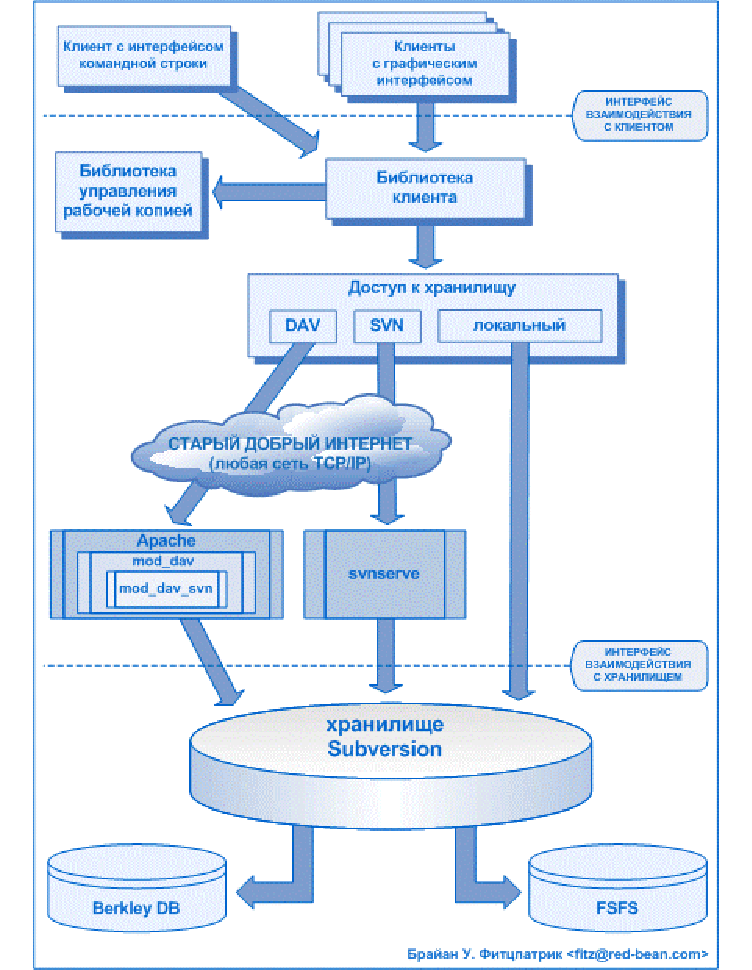
\includegraphics[width=0.5\textwidth]{SVNArchitecture.pdf}}
\end{frame}

\lecturenotes

На одной стороне схемы изображено хранилище Subversion, в котором хранится информация с версиями. На противоположной стороне показана программа-клиент Subversion, которая управляет локальными отражениями различных фрагментов этих данных (также называемыми «рабочими копиями»). Между этими сторонами проложены различные маршруты, проходящие через разные слои доступа к хранилищу. Некоторые из этих маршрутов используют компьютерные сети и сетевые сервера, чтобы достичь хранилища, в то время как другие маршруты в сети не нуждаются и ведут к хранилищу напрямую~\cite[с.~16--17]{VSwithSVN}. 

\begin{frame} \frametitle{Основные возможности Subversion}
  
  \begin{itemize}
  \item Контроль изменений каталогов
  \item Настоящая история версий
  \item Атомарная фиксация изменений
  \item Возможность конкурентной многопользовательской работы с хранилищем
  \item Метаданные с версиями
  \item Единый способ работы с данными
  \item Эффективные ветки и метки
  \end{itemize}
\end{frame}

\lecturenotes

Subversion предоставляет следующие возможности:
Контроль изменений каталогов 
Subversion использует «виртуальную» файловую систему с возможностями управления версиями, которая способна отслеживать изменения во времени целых структур каталогов. Под управление версиями попадают и файлы, и каталоги.

Настоящая история версий 
Subversion делает возможным добавление, удаление, копирование и переименование как файлов, так и каталогов. При этом каждый вновь добавленный файл начинает жизнь с чистого листа, сохраняя собственную историю изменений.

Атомарная фиксация изменений 
Каждый набор изменений либо попадает в хранилище целиком, либо не попадает туда вовсе. Это позволяет разработчикам создавать и фиксировать изменения логически оправданными кусками, предотвращая тем самым проблемы, которые могут возникать в тех случаях, когда только часть необходимых изменений помещается в хранилище успешно.

Возможность конкурентной многопользовательской работы с хранилищем
Поддержка конкурентной (в том числе одновременной, с изоляцией транзакций) многопользовательской работы с хранилищем и, в большинстве случаев, автоматическим слиянием изменений различных разработчиков (в рабочей копии);

Метаданные с версиями 
Каждый файл и каталог имеет собственный набор свойств, представленных в виде названия и значения. Вы можете создавать и сохранять любые необходимые пары названий свойств и их значений. Свойства файлов точно так же находятся под управлением версиями, как и их содержимое.

Единый способ работы с данными 
Subversion обнаруживает различия между файлами с помощью специального бинарного алгоритма, который одинаково работает как с текстовыми, так и с бинарными файлами. Файлы записываются в хранилище в сжатом виде независимо от их типа, а различия между отдельными версиями могут передаваться по сети в обоих направлениях.

Эффективные ветки и метки 
Плата за использование веток и меток не должна быть пропорциональна размеру проекта. Subversion создаёт ветки и метки путём простого копирования проекта, используя механизм, похожий на жёсткие ссылки в файловых системах. Благодаря этому, операции по созданию веток и меток занимают немного времени~\cite[с.~14--15]{VSwithSVN}.

\begin{frame} \frametitle{Дополнительные возможности Subversion}
  
  \begin{itemize}
  \item Различные варианты доступа к хранилищу (непосредственный доступ на диске, по собственному сетевому протоколу или через веб-сервер по протоколу WebDAV/DeltaV)
  \item Возможность зеркалирования хранилища
  \item Два возможных внутренних формата хранилища: база данных или набор обычных файлов
  \item Библиотеки для языков PHP, Python, Perl, Java позволяют встроить функциональность клиента Subversion в программы, написанные на этих языках
  \item Многоуровневая архитектура библиотек, изначально рассчитанная на клиент-серверную модель
  \end{itemize}
\end{frame}

\lecturenotes

Различные варианты доступа к хранилищу, в том числе, непосредственным доступом на диске, по собственному сетевому протоколу или через веб-сервер по протоколу WebDAV/DeltaV.
Возможность зеркалирования хранилища.
Два возможных внутренних формата хранилища: база данных или набор обычных файлов.
Библиотеки для языков PHP, Python, Perl, Java позволяют встроить функциональность клиента Subversion в программы, написанные на этих языках.
Многоуровневая архитектура библиотек, изначально рассчитанная на клиент-серверную модель~\cite{SVNMotu}.

\begin{frame} \frametitle{Недостатки Subversion}
  \begin{itemize}
  \item Проблемы при переименовании файлов
  \item Слабая поддержка слияния ветвей
  \item Невозможность удаления данных из хранилища
  \item Папка .svn в каждой папке
  \end{itemize}
\end{frame}

\lecturenotes

Проблемы при переименовании файлов
Subversion не всегда может правильно обработать операции переименования файлов, если одновременно с переименованием изменяется и содержимое файла. Проблемы могут также возникнуть, если файл, переименованный в локальной копии, кто-то другой изменил в хранилище. Часть этих проблем исправлена в версии 1.5, однако это решение пока не полное.

Слабая поддержка слияния ветвей
Также слабым местом Subversion считают операции слияния веток. До версии 1.5 все такие операции пользователям приходилось отслеживать вручную, с помощью подробных записей в журнале изменений. Начиная с версии 1.5 появилась базовая поддержка автоматического отслеживания слияний, которую разработчики планируют улучшить в последующих релизах. В настоящее время Subversion достаточно хорошо поддерживает типовые сценарии слияния; в более сложных случаях возможны проблемы. Рекомендуется организовать рабочий процесс так, чтобы избежать проблемных сценариев. Слияние переименованных файлов и директорий не поддерживается.

Невозможность удаления данных из хранилища
Информация, однажды помещённая в хранилище Subversion, остаётся там навсегда: файл можно удалить в текущей ревизии, но всегда есть возможность получить из хранилища одну из предыдущих ревизий, в которых файл существовал. Хотя сохранность прошлых ревизий и является, собственно, целью использования систем управления версиями, иногда бывает необходимо полностью удалить из хранилища информацию, попавшую туда по ошибке. В Subversion не предусмотрено для этого никакого штатного способа; единственная возможность заключается в создании дампа хранилища, его обработке штатной утилитой svndumpfilter и последующем восстановлении хранилища из дампа. Существуют также сторонние программы для автоматизации этого процесса, но, в любом случае, для выполнения этой операции требуется временное прекращение доступа к хранилищу и вмешательство администратора с привилегиями, достаточно высокими для того, чтобы полностью стереть старое хранилище и заменить его новым.

Папка .svn в каждой папке
засоряет файловую структуру проекта. Начиная с версии 1.7 в корне рабочей копии проекта создаётся одна директория .svn, метаданные в которой сохраняются с использованием SQLite~\cite{SVNWikipedia}.

\subsection{Git}

\begin{frame} \frametitle{Git}
  \begin{block}{}
    \alert{Git} --- распределённая система управления версиями. Проект был создан Линусом Торвальдсом для управления разработкой ядра Linux, первая версия выпущена 7 апреля 2005 года. На сегодняшний день его поддерживает Джунио Хамано
  \end{block}
\end{frame}

\begin{frame} \frametitle{Особенности Git}
  \begin{itemize}
  \item Снимки, а не различия
  \item Почти все операции выполняются локально
  \item Целостность Git
  \item Git только добавляет данные
  \item Три состояния
  \end{itemize}
\end{frame}

\lecturenotes

Снимки, а не различия
Основное отличие Git’а от любой другой СКВ, это подход Git’а к работе со своими данными. Концептуально, большинство других систем хранят информацию в виде списка изменений в файлах. Эти системы представляют информацию в виде набора файлов и изменений, сделанных в каждом файле, по времени. 
Git не хранит и не обрабатывает данные таким способом. Вместо этого, подход Git’а к хранению данных больше похож на набор снимков миниатюрной файловой системы. Каждый раз, когда вы делаете коммит, то есть сохраняете состояние своего проекта в Git’е, система запоминает, как выглядит каждый файл в этот момент, и сохраняет ссылку на этот снимок. Для увеличения эффективности, если файлы не были изменены, Git не запоминает эти файлы вновь, а только создаёт ссылку на предыдущую версию идентичного файла, который уже сохранён. Git представляет свои данные как, скажем, поток снимков.

Почти все операции выполняются локально
Для работы большинства операций в Git достаточно локальных файлов и ресурсов — в основном, системе не нужна никакая информация с других компьютеров в вашей сети. Если вы привыкли к ЦСКВ, где большинство операций имеют задержку из-за работы с сетью, то этот аспект Git’а заставит вас думать, что боги скорости наделили Git несказанной мощью. Так как вся история проекта хранится прямо на вашем локальном диске, большинство операций кажутся чуть ли не мгновенными.

Это также означает, что есть лишь небольшое количество действий, которые вы не сможете выполнить, если вы находитесь оффлайн или не имеете доступа к VPN в данный момент. Если вы в самолёте или в поезде и хотите немного поработать, вы сможете создавать коммиты без каких-либо проблем: когда будет возможность подключиться к сети, все изменения можно будет синхронизировать.

Целостность Git
В Git’е для всего вычисляется хеш-сумма, и только потом происходит сохранение. В дальнейшем обращение к сохранённым объектам происходит по этой хеш-сумме. Это значит, что невозможно изменить содержимое файла или директории так, чтобы Git не узнал об этом. Данная функциональность встроена в Git на низком уровне и является неотъемлемой частью его философии. Вы не потеряете информацию во время её передачи и не получите повреждённый файл без ведома Git.

Git только добавляет данные
Когда вы производите какие-либо действия в Git, практически все из них только добавляют новые данные в базу Git. Очень сложно заставить систему удалить данные либо сделать что-то, что нельзя впоследствии отменить. Как и в любой другой СКВ, вы можете потерять или испортить свои изменения, пока они не закоммичены, но после того, как вы закоммитите снимок в Git, будет очень сложно что-либо потерять, особенно, если вы регулярно синхронизируете свою базу с другим репозиторием

Три состояния
Git имеет три основных состояния, в которых могут находиться файлы: зафиксированном (committed), изменённом (modified) и подготовленном (staged). “Зафиксированный” значит, что файл уже сохранён в локальной базе. К изменённым относятся файлы, которые поменялись, но ещё не были зафиксированы. Подготовленные файлы — это изменённые файлы, отмеченные для включения в следующий коммит~\cite[с.~8-10]{ProGit}.

\begin{frame} \frametitle{Три секции проекта в Git}
  \centerline{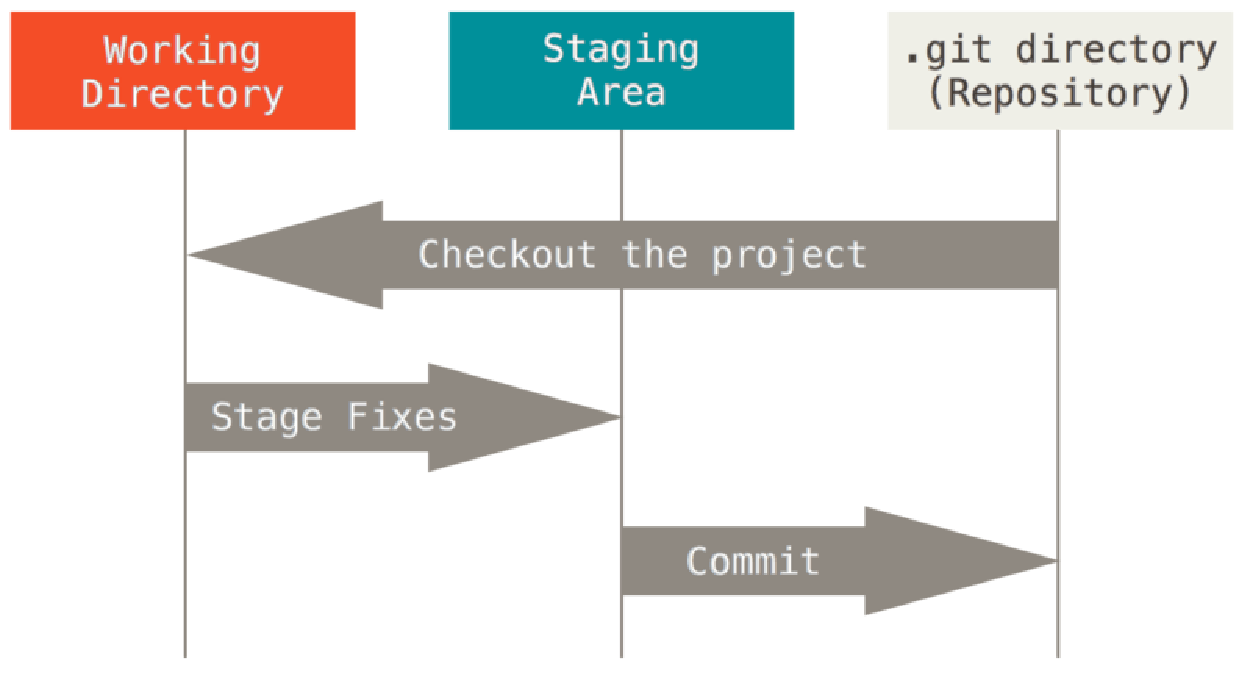
\includegraphics[width=0.9\textwidth]{GitSections.pdf}}
\end{frame}

\lecturenotes

У проекта Git есть три основные секции: Git-директория (Git directory), рабочая директория (working directory) и область подготовленных файлов (staging area).

Git-директория --- это то место, где Git хранит метаданные и базу объектов проекта. Это самая важная часть Git, и это та часть, которая копируется при клонировании репозитория с другого компьютера.
Рабочая директория является снимком версии проекта. Файлы распаковываются из сжатой базы данных в Git-директории и располагаются на диске, для того чтобы их можно было изменять и использовать.
Область подготовленных файлов — это файл, располагающийся в Git-директории, в нём содержится информация о том, какие изменения попадут в следующий коммит. Эту область ещё называют “индекс”, однако stage-область так же общепринятое название~\cite[с.~11]{ProGit}.

\begin{frame} \frametitle{Недостатки Git}
  
  \begin{itemize}
  \item Отсутствие сквозной нумерации коммитов монотонно непрерывно возрастающими целыми числами
  \item Некоторое неудобство для пользователей, переходящих с других VCS
  \item Использование для идентификации ревизий хешей SHA1 не всегда бывает удобно
  \item Большие накладные расходы при работе с проектами, в которых делаются многочисленные несвязанные между собой изменения файлов
  \item Отсутствие отдельной команды переименования/перемещения файла, которая отображалась бы в истории как соответствующее единое действие
  \item Большие накладные расходы при работе с проектами, в которых делаются многочисленные несвязанные между собой изменения файлов
  \end{itemize}
\end{frame}

\lecturenotes

Отсутствие сквозной нумерации коммитов монотонно непрерывно возрастающими целыми числами. Во многих проектах используется автоматическое получение номера этой версии (например, командой svnversion), построение .H файла на основе этого числа, и далее его использование при создании штампа версии исполняемого файла, некоторых вшитых в него строк и так далее.

Некоторое неудобство для пользователей, переходящих с других VCS. Команды git, ориентированные на наборы изменений, а не на файлы, могут вызвать недоумение у пользователей, привыкших к файл-ориентированным VCS, таким как SVN. Например, команда «add», которая в большинстве систем управления версиями производит добавление файла к проекту, в git подготавливает к фиксации сделанные в файлах изменения. При этом сохраняется не патч, описывающий изменения, а новая версия целевого файла.

Использование для идентификации ревизий хешей SHA1, что приводит к необходимости оперировать длинными строками вместо коротких номеров версий, как во многих других системах (хотя в командах допускается использование неполных хеш-строк).

Большие накладные расходы при работе с проектами, в которых делаются многочисленные несвязанные между собой изменения файлов. При работе в таком режиме размеры наборов изменений становятся достаточно велики и происходит быстрый рост объёма репозиториев.

Отсутствие отдельной команды переименования/перемещения файла, которая отображалась бы в истории как соответствующее единое действие. Существующий скрипт git mv фактически выполняет переименование, копирование файла и удаление его на старом месте, что требует специального анализа для определения, что в действительности файл был просто перенесён (этот анализ выполняется автоматически командами просмотра истории). Однако, учитывая тот факт, что наличие специальной команды для переименования/перемещения файлов технически не вынуждает пользователя использовать именно её (и, как следствие, в этом случае возможны разрывы в истории), поведение git может считаться преимуществом.

Система работает только с файлами и их содержимым, и не отслеживает пустые каталоги~\cite{GitWikipedia}.

\subsection{Mercurial}

\begin{frame} \frametitle{Mercurial}
  \begin{block}{}
    \alert{Mercurial, он же Hg (от обозначения химического элемента ртути)} --- кроссплатформенная распределённая система управления версиями, разработанная для эффективной работы с очень большими репозиториями кода
  \end{block}
\end{frame}

\begin{frame} \frametitle{Особенности Mercurial}
  
  \begin{itemize}
  \item Прост в изучении и использовании
  \item Легковесный
  \item Превосходно масштабируется
  \item Легко настраивается под конкретные нужды
  \end{itemize}
\end{frame}

\lecturenotes

Mercurial обладает уникальным набором свойств, позволяющим выбрать его в качестве наиболее подходящей системы контроля версий: Прост в изучении и использовании, Легковесный, Превосходно масштабируется, Легко настраивается под конкретные нужды.

Mercurial предоставляет единообразную и последовательную систему команд и функций, что позволяет руководствоваться небольшим набором общих правил вместо того, чтобы учить массу исключений.

В небольших проектах вы можете начать работу с Mercurial в считанные минуты. Создание новых веток и изменений, распространение изменений (как локально, так и по сети), операции с историей и статусом — всё это работает быстро. Mercurial старается быть незаметным и не путаться под вашими ногами, не требует от вас больших умственных усилий и совершает свои операции невероятно быстро.

Mercurial применяется не только в маленьких проектах, его используют и в проектах с сотнями и тысячами разработчиков, проектах, которые содержат десятки тысяч файлов и сотни мегабайт исходного кода.

Если вам не хватает базовой функциональности Mercurial, то её легко расширить. Mercurial хорошо подходит для задач скриптинга, его понятное устройство и реализация на языке Python позволяет легко добавлять новые возможности в виде расширений. Существует большое количество популярных и полезных расширений, охватывающих спектр задач от помощи в нахождении ошибок до улучшения производительности~\cite[с.~6--7]{MercurialOReilly}.

\begin{frame} \frametitle{Модель данных в Mercurial}
  \begin{block}{}
    \alert{Ревизия (changeset)} --- это сущность, описывающая изменения в каких-либо файлах. Эта сущность хранит информацию о своём авторе, времени создания, изменениях в файлах и о родительских ревизиях. 
  \end{block}

  \begin{itemize}
  \item Ревизия идентифицирует не только себя, но и всю свою историю
  \item Ревизии организовывают ориентированный ациклический граф
  \item Существуют две специальные ревизии: null (ревизия-родитель) и tip (самая последняя ревизия)
  \end{itemize}
\end{frame}

\lecturenotes

Ревизия (changeset) - это сущность, описывающая изменения в каких-либо файлах. Эта сущность хранит информацию о своём авторе, времени создания, изменениях в файлах и о родительских ревизиях (которых может быть одна в случае обычной ревизии и две в случае слияния). Кстати, подсчёт 40-цифрового 16-ричного sha1-хеша, которым идентифицируется ревизия, учитывает все эти значения - таким образом каждая ревизия идентифицирует не только себя, но и всю свою историю.

Эти ревизии (благодаря наличию у себя родителей) организовывают ориентированный ациклический граф (от ревизии 0 и до существующих голов), который может разветвиться в любом месте.

Головы - это ревизии, у которых (ещё) нет детей, конечные точки графа.

При этом существуют две специальные ревизии - null (ревизия-родитель самой первой ревизии под номером 0) и tip (самая последняя ревизия, в случае наличия нескольких голов выбирается в зависимости от обстоятельств)~\cite{MercurialSolovyov}.

\begin{frame} \frametitle{Возможности Mercurial}
  
  \begin{itemize}
  \item Обладает превосходной производительностью
  \item Репозиторий Mercurial не требует операций по техническому обслуживанию
  \item Используются стандартные протоколы для обмена данными между репозиториями (http(s), ssh)
  \item Возможен импорт истории изменений из репозитория Subversion или Git
  \end{itemize}
\end{frame}

\lecturenotes

Git очень быстр. В некоторых случаях он быстрее, чем Mercurial (по крайней мере под Linux), а в других быстрее оказывается Mercurial. Однако под Windows как производительность, так и общий уровень поддержки, во время написания этой книги у Git гораздо хуже, чем у Mercurial.

В то время как репозиторий Mercurial не требует операций по техническому обслуживанию, репозиторий Git требует частых ручных «перепаковок» собственных метаданных. Если этого не делать, производительность начинает падать, наряду с увеличением объёма занимаемого дискового пространства. Дисковый массив сервера, содержащего несколько Git репозиториев, по отношению к которым не выполняется строгое правило частой «перепаковки», рано или поздно забивается под завязку, в результате чего процесс ежедневного резервного копирования легко может занимать более 24 часов. 

Использование абсолютно стандартных протоколов для обмена данными между репозиториями: http (и https), ssh или, на худой конец, аттачами в email.
При этом никаких усилий или отдельных демонов не требуется. ssh работает без всякой настройки, а http-часть идёт в комплекте и требует веб-сервера, могущего cgi/fastcgi/wsgi (на выбор). Протоколы работы по ним очень похожи - локальный и удалённый меркуриалы обмениваются bundle’ами, сжатыми файлами с группой ревизий.

Mercurial может импортировать историю изменений из репозитория Subversion. Возможен и обратный процесс. Это делает возможным прощупать почву и использовать Mercurial и Subversion одновременно, прежде чем решить, осуществлять переход или нет. Преобразование истории — пошаговый процесс, так что вы можете осуществить начальное преобразование, а потом вносить новые изменения.
Mercurial предоставляет возможность импорта истории версий из репозитория Git~\cite[с.~7--9]{MercurialOReilly}.

\begin{frame} \frametitle{Недостатки Mercurial}
  
  \begin{itemize}
  \item Невозможно размещать и раздельно использовать несколько проектов в одном репозитории
  \item Нет возможности слияния двух родительских веток
  \item Использование плагинов, а не скриптов
  \end{itemize}
\end{frame}

\lecturenotes

Некоторые ожидают что с помощью hg можно размещать и раздельно использовать несколько проектов в одном репозитории. В действительности, это не то, ради чего hg был создан. В частности, это означает, что вы не можете получить из репозитория только один каталог~\cite{MercurialWiki}.

Один из существенных недостатков Mercurial заключается в том, что в отличии от Git в ней нельзя объединить две родительские ветки, так как Mercurial использует систему плагинов, а не поддержку скриптов~\cite{MercurialTD}.

\section{Коллективная разработка с использованием систем контроля версий}

\section{Интеграция систем контроля версий в проектную инфраструктуру}


\begin{thebibliography}{99}
\bibitem{Atlassian} \href{https://www.atlassian.com/git/tutorials/what-is-version-control}{What is version control | Atlassian Git Tutorial}
\bibitem{ProGit} Scott Chacon Pro Git 1st Edition. Apress, 2009
\bibitem{VSwithSVN} 	Brian Fitzpatrick, C. Pilato, Ben Collins-Sussman Version Control with Subversion. O'Reilly Media, 2009
\bibitem{SVNMotu} \href{http://henry-motu.org.ua/2010/10/02/subversion-svobodnaja-sistema-upravkenija-versijam/}{Subversion --- свободная система управления версиями | Henry Motu}
\bibitem{SVNWikipedia} \href{https://ru.wikipedia.org/wiki/Subversion}{Subversion --- Википедия}
\bibitem{GitWikipedia} \href{https://ru.wikipedia.org/wiki/Git}{Git --- Википедия}
\bibitem{MercurialOReilly} Bryan O'Sullivan Mercurial: The Definitive Guide. O'Reilly Media, 2009
\bibitem{MercurialSolovyov} \href{https://solovyov.net/blog/2008/mercurial-basics/}{solovyov.net: Mercurial: основы}
\bibitem{MercurialWiki} \href{https://www.mercurial-scm.org/wiki/RussianUnderstandingMercurial}{Understanding Mercurial --- Mercurial}
\bibitem{MercurialTD} \href{https://biz30.timedoctor.com/ru/cистема-контроля-версий/}{Система контроля версий (cvs) 2017 - Сравниваем: Git, SVN, Mercurial}
\end{thebibliography}

\end{document}

%%% Local Variables: 
%%% mode: TeX-pdf
%%% TeX-master: t
%%% End: 
